
% UC... specificare App o Server -> UCA / UCS

%\centering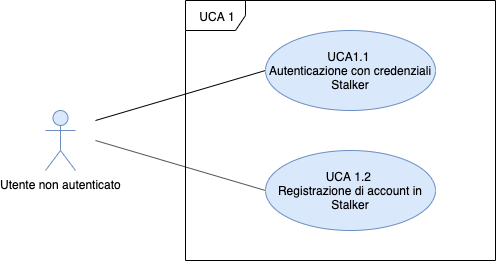
\includegraphics[scale=0.8]{sezioni/UseCase/Immagini/Panoramica.png}
\section{UCS 4}%kite level
\begin{itemize}
    \item \textbf{Nome:} Modifica parametri dell'organizzazione
    \item \textbf{Attori primari:} Amministratore gestore
    \item \textbf{Precondizione:} L’amministratore dispone di almeno un'organizzazione.
    \item \textbf{Postcondizione:} L’amministratore ha modificato i parametri desiderati dell'organizzazione e le modifiche sono state salvate nel sistema.
    \item \textbf{Scenario principale:} L'amministratore deve scegliere l'organizzazione che vuole modificare, selezionare la funzionalità di modifica dell'organizzazione e quindi procedere con il cambiamento dei dati.
    \item \textbf{Flusso di eventi:}
    \begin{enumerate}
        \item UCS 3 Selezione dell'organizzazione;
        \item L'amministratore seleziona la funzionalità di modifica dell'organizzazione;
        \item UCS 4.1 L'amministratore ha la possibilità di modificare i campi delle informazioni dell’organizzazione;
        \item UCS 5 L'amministratore ha la possibilità di modificare i luoghi di tracciamento dell’organizzazione;
        \item L'amministratore seleziona la funzionalità per il salvataggio delle modifiche apportate;
    \end{enumerate}
    \item \textbf{Inclusioni:}
    \begin{itemize}
        \item UCS 3;
        \item UCS 4.1;
        \item UCS 4.2;
        \item UCS 4.4;
    \end{itemize}
    \item \textbf{Estensioni:}
    \begin{itemize}
        \item UCS ERRORE.4.1 Annullamento modifiche ai parametri dell'organizzazione
    \end{itemize}
\end{itemize}

\subsection{UCS 4.1}%sea level
\begin{itemize}
    \item \textbf{Nome:} Modifica dei dati dell'organizzazione
    \item \textbf{Attori primari:} Amministratore gestore
    \item \textbf{Precondizione:} L'amministratore si trova nella sezione di modifica dei parametri dell'organizzazione
    \item \textbf{Postcondizione:} L'amministratore ha modificato i dati desiderati all'interno dell’organizzazione.
    \item \textbf{Scenario principale:} L'amministratore modifica i dati dell'organizzazione desiderati.
    \item \textbf{Flusso di eventi:}
    \begin{enumerate}
        \item L'amministratore ha la possibilità di modificare il nome dell'organizzazione UCS 4.1.1;
        \item L'amministratore ha la possibilità di modificare l'immagine dell'organizzazione UCS 4.1.2;
        \item L'amministratore ha la possibilità di modificare la descrizione dell'organizzazione UCS 4.1.3;
        \item L'amministratore ha la possibilità di modificare l'indirizzo dell'organizzazione UCS 4.1.4;
    \end{enumerate}
    \item \textbf{Estensioni:}
    \begin{itemize}
        \item UCS ERRORE.4.2 Il nome dell 'organizzazione inserito non rispetta i vincoli imposti
        \item UCS ERRORE.4.3 L'immagine dell'organizzazione scelta non rispetta i vincoli imposti
    \end{itemize}
    \item \textbf{Inclusioni:}
    \begin{enumerate}
	    \item UCS 4.1.1;
	    \item UCS 4.1.2;
	    \item UCS 4.1.3;
	    \item UCS 4.1.4;
    \end{enumerate}
\end{itemize}

\subsubsection{UCS 4.1.1}%fish level
\begin{itemize}
\item \textbf{Nome:} Modifica del nome dell'organizzazione
\item \textbf{Attori primari:} Amministratore gestore
\item \textbf{Precondizione:} L'amministratore gestore si trova nella sezione di modifica dei parametri dell'organizzazione.
\item \textbf{Postcondizione:} L'amministratore ha inserito un nome per l'organizzazione che rispetti i vincoli imposti e non sia già presente nel sistema.
\item \textbf{Estensioni:}
\begin{enumerate}
    \item UCS Errore.4.? Il nome dell'organizzazione inserito non rispetta i vincoli;
    \item UCS Errore.1.? Il nome dell'organizzazione inserito è già presente nel sistema;
\end{enumerate}
\end{itemize}

\subsubsection{UCS 4.1.2}%fish level
\begin{itemize}
\item \textbf{Nome:} Modifica dell'immagine dell'organizzazione
\item \textbf{Attori primari:} Amministratore gestore
\item \textbf{Precondizione:} L'amministratore gestore si trova nella sezione di modifica dei parametri dell'organizzazione.
\item \textbf{Postcondizione:} L'amministratore ha selezionato un'immagine valida per l'organizzazione
\item \textbf{Flusso di eventi:}
\begin{enumerate}
    \item L'amministratore seleziona la funzionalità di scelta dell'immagine;
    \item Seleziona l'immagine da impostare come immagine dell'organizzazione;
    \item Conferma la scleta;
\end{enumerate}
\item \textbf{Estensioni:}
\begin{enumerate}
    \item UCS Errore.4.? L'immagine selezionata non è valida;
\end{enumerate}
\end{itemize}

\subsubsection{UCS 4.1.3}%fish level
\begin{itemize}
\item \textbf{Nome:} Modifica della descrizione dell'organizzazione
\item \textbf{Attori primari:} Amministratore gestore
\item \textbf{Precondizione:} L'amministratore gestore si trova nella sezione di modifica dei parametri dell'organizzazione.
\item \textbf{Postcondizione:} L'amministratore ha inserito una descrizione che rispetti i vincoli imposti.
\item \textbf{Estensioni:}
\begin{enumerate}
    \item UCS Errore.4.? La descrizione inserita non rispetta i vincoli;
\end{enumerate}
\end{itemize}

\subsubsection{UCS 4.1.4}%fish level
\begin{itemize}
\item \textbf{Nome:} Modifica dell'indirizzo dell'organizzazione
\item \textbf{Attori primari:} Amministratore gestore
\item \textbf{Precondizione:} L'amministratore gestore si trova nella sezione di modifica dei parametri dell'organizzazione.
\item \textbf{Postcondizione:} L'amministratore ha inserito un indirizzo valido che rispetti i vincoli imposti.
\item \textbf{Flusso di eventi:}
\begin{enumerate}
    \item L'amministratore inserisce una parola tra: via/viale/piazza;
    \item L'amministratore inserisce il nome della via/viale/piazza dell'azienda;
    \item L'amministratore inserisce il numero civico;
    \item Se serve, l'amministratore inserisce la lettera che identifica l'azienda dagli altri edifici che condividono lo stesso numero civico con essa.
\end{enumerate}
\item \textbf{Estensioni:}
\begin{enumerate}
    \item UCS Errore.4.? L'indirizzo inserito non rispetta i vincoli imposti;
\end{enumerate}
\end{itemize}